\subsection{Análisis de tecnologías}

En esta instancia del informe, se procede a comparar compuertas lógicas del tipo NOR de diversas tecnologías. Para ello se vale de las hojas de datos de las compuertas \href{http://www.ti.com/lit/ds/symlink/sn74hc02.pdf}{74HC02}, \href{http://www.ti.com/lit/ds/symlink/sn74hct02.pdf}{74HCT02} y \href{http://www.ti.com/lit/ds/symlink/sn74ls02.pdf}{74LS02}. Previo a dicho análisis, cabe detallar cada una de las tecnologías. Primero, se encuentra el 74HC02, siendo este, como su nombre lo indica, del tipo HC, cuyas siglas significan ``High-speed CMOS'', tecnología caracterizada por ser de baja potencia y alta velocidad. Luego se encuentra el 74HCT02, siendo HCT una variación de las HC. Esta denominación proviene de las mismas siglas previamente mencionadas, solo que ademas posee compatibilidad con la tecnología conocida como ``logica transistor–transistor'' (TTL). En otras palabras, este tipo de compuertas puede operar bajo dicho estándar de tensiones, tanto de alimentación como de input.\footnote{``Logic family'', En.wikipedia.org, 2019. [Online]. Available: \url{https://en.wikipedia.org/wiki/Logic\_family\#HC\_logic}. [Accessed: 21- Sep- 2019].} Finalmente se encuentra el 74LS02, cuyas siglas provienen de ``Low~-power Schottky''. Los integrados de esta familia se caracterizan por estar hechos con tecnología TTL.\footnote{``Serie 7400'', Es.wikipedia.org, 2019. [Online]. Available: \url{https://es.wikipedia.org/wiki/Serie\_7400}. [Accessed: 21- Sep- 2019].} Se destaca que este último, a diferencia de los dos primeros, se caracteriza por ser fabricado mediante el uso de tecnología BJT.

Analizando las respectivas hojas de datos, se recopila información sobre los  valores aceptables de señal, tanto de entrada como de salida. Es así que se realiza la siguiente tabla:
\begin{table}[H]
\centering
\begin{tabular}{c|c|c|c|c|c|c|c|}
\cline{2-8}
                               & $\mathbf{V_{CC}}$ \textbf{[V]} & \multicolumn{2}{c|}{\textbf{74HC02}}  & \multicolumn{2}{c|}{\textbf{74HCT02}} & \multicolumn{2}{c|}{\textbf{74LS02}} \\ \cline{3-8} 
                               &              & \textbf{Min. [V]} & \textbf{Max. [V]} & \textbf{Min. [V]} & \textbf{Max. [V]} & \textbf{Min. [V]} & \textbf{Max. [V]}	\\ \hline
\multicolumn{1}{|c|}{}         & 2            & 1.9           & -            & -             & -            & -          & -            \\  
\multicolumn{1}{|c|}{$\mathbf{V_{OH}}$} & 4.5          & 4.4           & -            & 3.84          & -            & 2.7            & -            \\  
\multicolumn{1}{|c|}{}         & 6            & 5.9           & -            & -             & -            & -            & -            \\ \hline
\multicolumn{1}{|c|}{}         & 2            & -             & 0.1          & -             & -            & -            & -          \\
\multicolumn{1}{|c|}{$\mathbf{V_{OL}}$} & 4.5          & -             & 0.1          & -             & 0.33         & -            & 0.5            \\
\multicolumn{1}{|c|}{}         & 6            & -             & 0.1          & -             & -            & -            & -            \\ \hline
\multicolumn{1}{|c|}{}         & 2            & 1.5           & -            & -             & -            & -            & -            \\ 
\multicolumn{1}{|c|}{$\mathbf{V_{IH}}$}  & 4.5          & 3.15          & -            & 2             & -            & 2            & -            \\ 
\multicolumn{1}{|c|}{}         & 6            & 4.2           & -            & -             & -            & -            & -            \\ \hline
\multicolumn{1}{|c|}{}         & 2            & -             & 0.5          & -             & -            & -            & -            \\ 
\multicolumn{1}{|c|}{$\mathbf{V_{IL}}$} & 4.5          & -             & 1.35         & -             & 0.8          & -            & 0.8          \\ 
\multicolumn{1}{|c|}{}         & 6            & -             & 1.8          & -             & -            & -            & -            \\ \hline
\end{tabular}
\centering
\caption{Tabla de valores de entrada y salida.}
\label{tabla:vinout}
\end{table}

Con la información que se ha detallado, se procede a analizar el margen de ruido, tanto para los niveles altos (high), como para los bajos (low), al combinar tecnologías HC y LS, siendo este calculado de la forma
\begin{equation*}
\begin{aligned}
		NM_{High}=\ & V_{OH} - V_{IH} \\
		NM_{Low}=\ & V_{IL} - V_{OL} 
\end{aligned}
\end{equation*}

Nuevamente se decide plasmar los resultados en una tabla:
\begin{table}[H]
\centering
\begin{tabular}{ccccc}
\hline
\textbf{In} & \textbf{Out} & $\mathbf{V_{CC}}$ \textbf{[V]} & $\mathbf{NM_{High}}$ \textbf{[V]} & $\mathbf{NM_{Low}} $\textbf{[V]} \\ \hline
74LS02      & 74HC02       & 4.5                            & 2.4                               & 0.7                              \\ 
74HC02      & 74LS02       & 4.5                              & -0.45                               & 0.85                                \\ \hline
\end{tabular}
\caption{Margen de ruido para combinaciones de tecnologías HC y LS.}
\label{tabla:nm}
\end{table}

Luego, se procede a representar de una forma más clara los datos obtenidos en la Tabla (\ref{tabla:vinout}) y (\ref{tabla:nm}).  

\begin{figure}[H]
\begin{center}
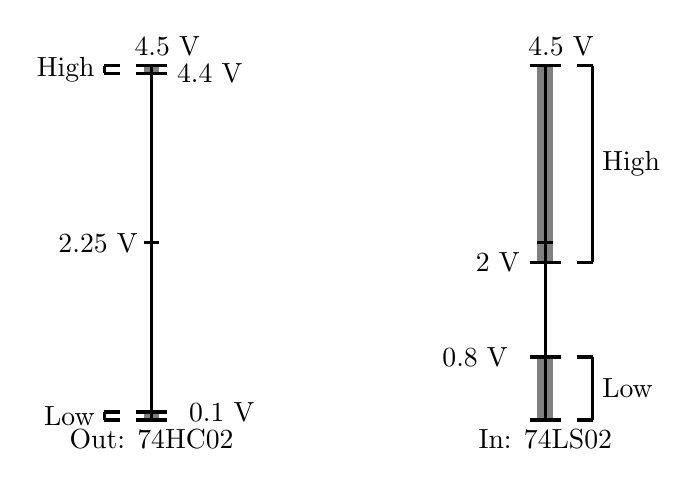
\begin{tikzpicture}[yscale=1]
	\node [below] at (0,0) {Out: 74HC02};
	
	\draw[-][draw=gray, line width=2mm] (0,4.4) -- (0,4.5);
	\draw[-][draw=gray, line width=2mm] (0,0) -- (0,0.1);	
	\draw[-][draw=black, very thick] (-0.2,4.4) -- (0.2,4.4);
	\draw[-][draw=black, very thick] (-0.2,0.1) -- (0.2,0.1) node[label=right:0.1 V](){};

	\draw[-][draw=black, very thick] (0,0) -- (0,4.5);
	\draw[-][draw=black, very thick] (-0.1,2.25) -- (0.1,2.25) node[label=left:2.25 V](){};
	\draw[-][draw=black, very thick] (-0.2,0) -- (0.2,0);
	\draw[-][draw=black, very thick] (-0.2,4.5) -- (0.2,4.5);
	
	\draw[-][draw=black, very thick] (-0.4,4.5) -- (-0.6,4.5);
	\draw[-][draw=black, very thick] (-0.6,4.5) -- (-0.6,4.4);
	\draw[-][draw=black, very thick] (-0.4,4.4) -- (-0.6,4.4);
	\node [left] at (-0.6,4.45) {High};
	\node [above] at (0.2,4.5) {4.5 V};
	\node [right] at (0.2,4.4) {4.4 V};
	
	\draw[-][draw=black, very thick]	 (-0.4,0) -- (-0.6,0);
	\draw[-][draw=black, very thick]	 (-0.4,0.1) -- (-0.6,0.1);
	\draw[-][draw=black, very thick]	 (-0.6,0) -- (-0.6,0.1);
	\node [left] at (-0.6,0.05) {Low};
	
	
	\node [below] at (5,0) {In: 74LS02};
	\draw[-][draw=gray, line width=2mm] (5,0) -- (5,0.8);
	\draw[-][draw=gray, line width=2mm] (5,2) -- (5,4.5);
	\draw[-][draw=black, very thick] (5.2,0.8) -- (4.8,0.8) node[label=left:0.8 V](){};
	\node [above] at (5.2,4.5) {4.5 V};
	
	\draw[-][draw=black, very thick] (5,0) -- (5,4.5);
	\draw[-][draw=black, very thick] (4.9,2.25) -- (5.1,2.25);
	\draw[-][draw=black, very thick] (4.8,0) -- (5.2,0);
	\draw[-][draw=black, very thick] (4.8,4.5) -- (5.2,4.5);
	\draw[-][draw=black, very thick] (5.4,0) -- (5.6,0);
	\draw[-][draw=black, very thick] (4.8,2) -- (5.2,2);
	\draw[-][draw=black, very thick] (5.4,0.8) -- (5.6,0.8);
	\draw[-][draw=black, very thick] (5.6,0) -- (5.6,0.8);
	\node [right] at (5.6,0.4) {Low};

	\draw[-][draw=black, very thick] (5.4,2) -- (5.6,2);
	\node [left] at (4.8,2) {2 V};	
	\draw[-][draw=black, very thick] (5.4,4.5) -- (5.6,4.5);
	\draw[-][draw=black, very thick] (5.6,2) -- (5.6,4.5);
	\node [right] at (5.6,3.25) {High};	
\end{tikzpicture}
\end{center}
\caption{Comparación de tecnologías con HC a la salida y LS a la entrada.}
\label{fig:hcls}
\end{figure}

\begin{figure}[H]
\begin{center}
\begin{tikzpicture}[yscale=1]
	\node [below] at (0,0) {Out: 74LS02};
	
	\draw[-][draw=gray, line width=2mm] (0,2.7) -- (0,4.5);
	\draw[-][draw=gray, line width=2mm] (0,0) -- (0,0.5);	
	\draw[-][draw=black, very thick] (-0.2,2.7) -- (0.2,2.7);
	\draw[-][draw=black, very thick] (-0.2,0.5) -- (0.2,0.5) node[label=right:0.5 V](){};

	\draw[-][draw=black, very thick] (0,0) -- (0,4.5);
	\draw[-][draw=black, very thick] (-0.1,2.25) -- (0.1,2.25) node[label=left:2.25 V](){};
	\draw[-][draw=black, very thick] (-0.2,0) -- (0.2,0);
	\draw[-][draw=black, very thick] (-0.2,4.5) -- (0.2,4.5);
	
	\draw[-][draw=black, very thick] (-0.4,4.5) -- (-0.6,4.5);
	\draw[-][draw=black, very thick] (-0.6,4.5) -- (-0.6,2.7);
	\draw[-][draw=black, very thick] (-0.4,2.7) -- (-0.6,2.7);
	\node [left] at (-0.6,3.6) {High};
	\node [above] at (0.2,4.5) {4.5 V};
	
	\node [right] at (0.2,2.5) {2.7 V};
	
	\draw[-][draw=black, very thick]	 (-0.4,0) -- (-0.6,0);
	\draw[-][draw=black, very thick]	 (-0.4,0.5) -- (-0.6,0.5);
	\draw[-][draw=black, very thick]	 (-0.6,0) -- (-0.6,0.5);
	\node [left] at (-0.6,0.25) {Low};
	
	
	\node [below] at (5,0) {In: 74HC02};
	\draw[-][draw=gray, line width=2mm] (5,0) -- (5,1.35);
	\draw[-][draw=gray, line width=2mm] (5,3.15) -- (5,4.5);
	\draw[-][draw=black, very thick] (5.2,1.35) -- (4.8,1.35) node[label=left:1.35 V](){};
	\node [above] at (5.2,4.5) {4.5 V};
	
	\draw[-][draw=black, very thick] (5,0) -- (5,4.5);
	\draw[-][draw=black, very thick] (4.9,2.25) -- (5.1,2.25) node[label=right:2.25 V](){};
	\draw[-][draw=black, very thick] (4.8,0) -- (5.2,0);
	\draw[-][draw=black, very thick] (4.8,4.5) -- (5.2,4.5);
	\draw[-][draw=black, very thick] (5.4,0) -- (5.6,0);
	\draw[-][draw=black, very thick] (5.2,3.15) -- (4.8,3.15);
	\draw[-][draw=black, very thick] (5.4,1.35) -- (5.6,1.35);
	\draw[-][draw=black, very thick] (5.6,0) -- (5.6,1.35);
	\node [right] at (5.6,0.675) {Low};

	\draw[-][draw=black, very thick] (5.4,3.15) -- (5.6,3.15);
		\draw[-][draw=black, very thick] (5.4,4.5) -- (5.6,4.5);
	\draw[-][draw=black, very thick] (5.6,3.15) -- (5.6,4.5);
	\node [right] at (5.6,3.825) {High};
	
	\node [left] at (4.8,3.35) {3.15 V};	
	
	\draw[pattern=custom north west lines, hatchcolor=red, hatchspread=6pt] (0,2.7) rectangle (5,3.15);	
	
\end{tikzpicture}
\end{center}
\caption{Comparación de tecnologías con LS a la salida y HC a la entrada.}
\label{fig:lshc}
\end{figure}

A la hora de conectar una compuerta con otra, es deseable que los rangos de valores validos de salida sean menores que los de entrada, ya que de esta forma se garantiza que cualquier salida sea interpretada adecuadamente por la siguiente etapa. Por consiguiente, de la Tabla (\ref{tabla:nm}) se destaca el valor negativo de $NM_{High}$ al colocar las compuertas de tecnología HC a la salida de una LS, detalle que se vuelve a observar en la Figura (\ref{fig:lshc}). Al conectar los dispositivos como se mencionó anteriormente, se pone en evidencia que existe la posibilidad de que tensiones de salida, que se consideran altas, caigan en un margen en el cual la siguiente compuerta las considera como valores imprecisos, es decir, que no actúa frente a estos. Particularmente, tensiones de salida desde $2.7 \ V$ hasta $3.15 \ V$ sin incluir, que son considerados como activos altos para la tecnología LS, no lo son para la HC. Por lo tanto, no es conveniente realizar dicha conexión, ya que se podría generar perdida de datos.

Es así que se decide observar dicho factor. Se diseñó un circuito que represente lo mostrado en la Figura (\ref{fig:lshc}), con las compuertas mencionadas, variando la entrada del circuito con una rampa periódica que varía desde los $0 \ V$ hasta los $5 \ V$. De esta forma se obtuvieron las siguientes mediciones:

\begin{figure}[H]
\centering
	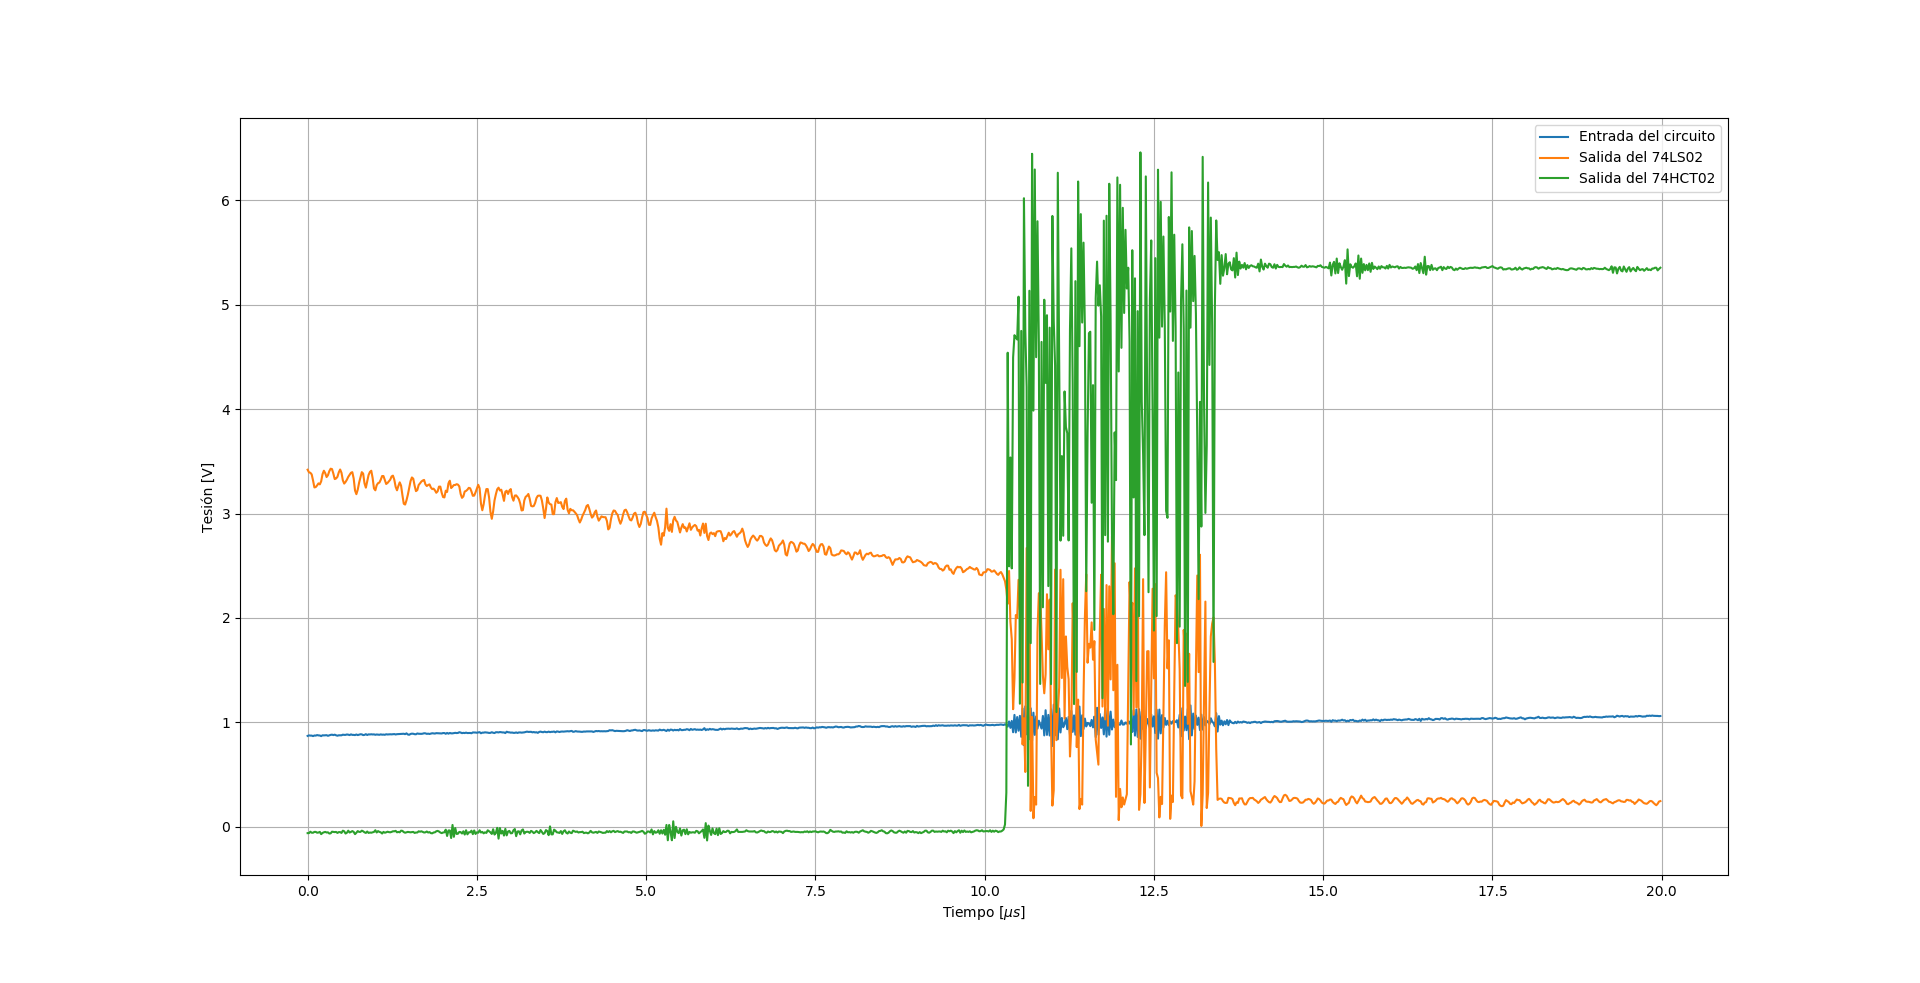
\includegraphics[width=0.8\textwidth]{ImagenesEjercicio2/scope_17_1.png}
\end{figure}
\vspace*{-2cm}
\begin{figure}[H]
\centering
	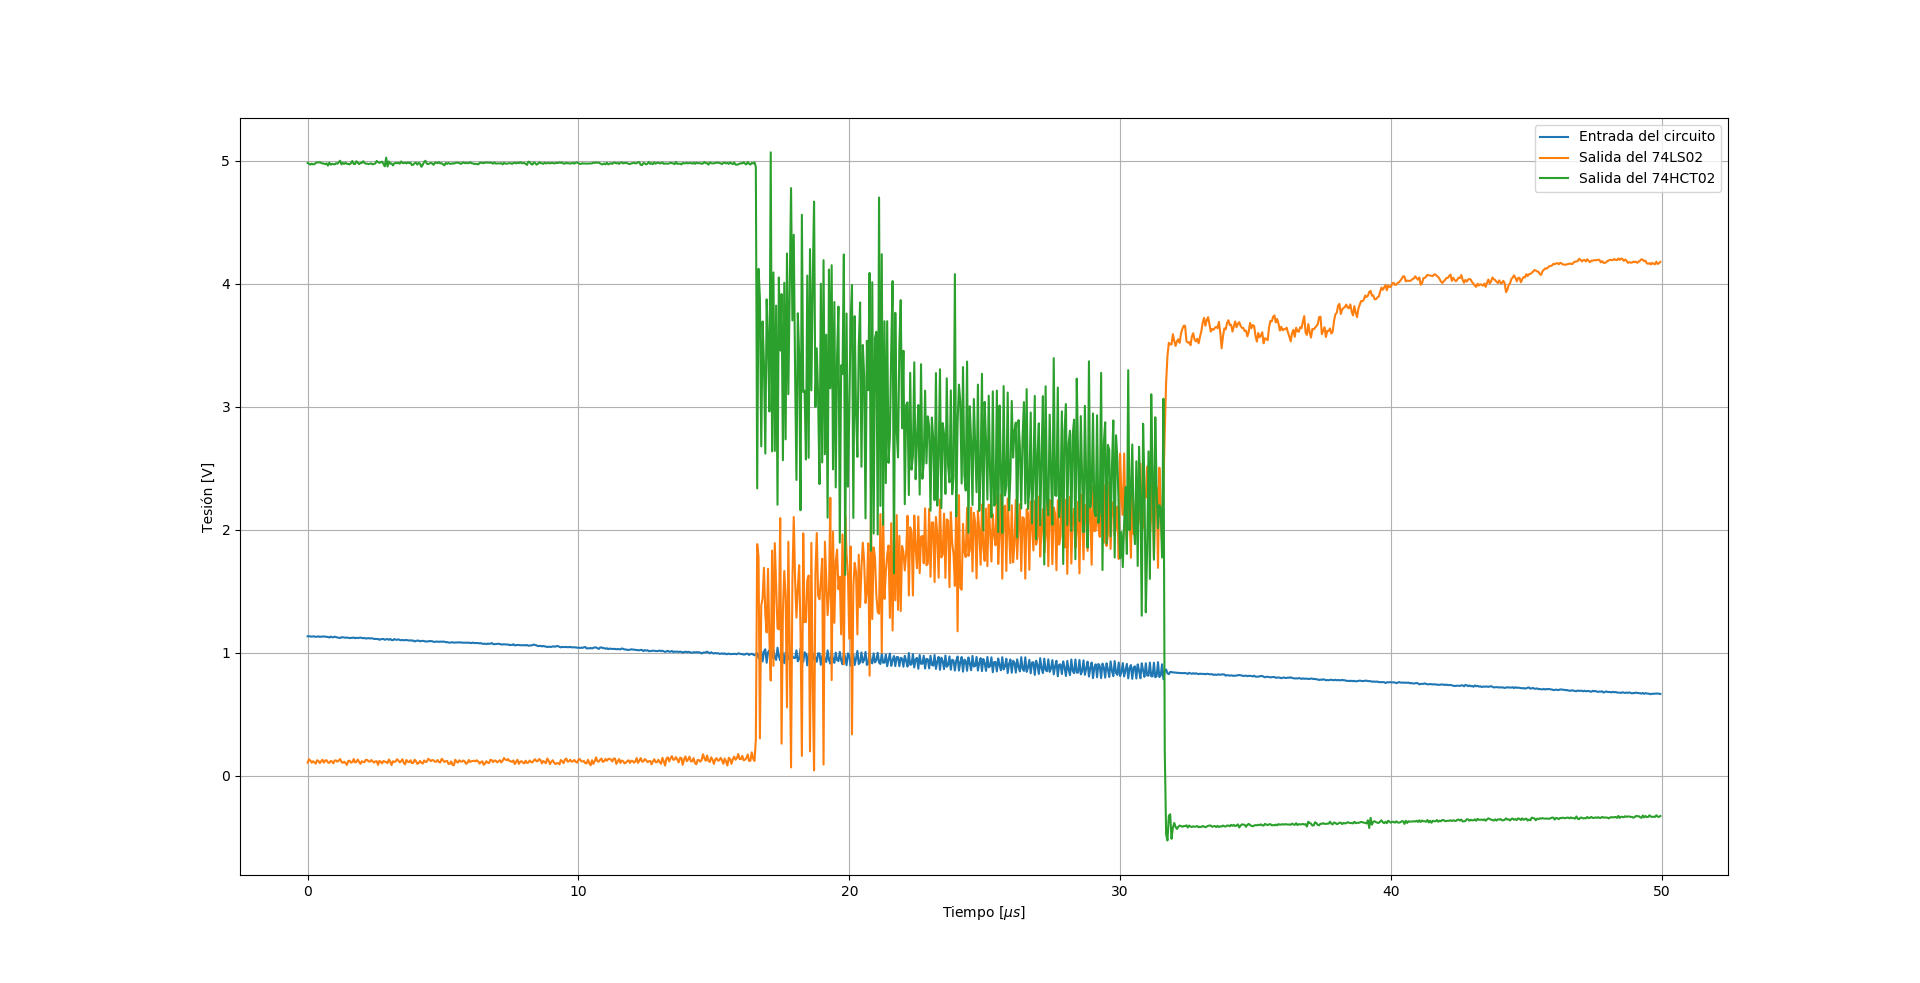
\includegraphics[width=0.8\textwidth]{ImagenesEjercicio2/scope_18_1.png}	
\caption{Entrada del circuito , salida del 74LS02 y salida del 74HC02.}
\label{fig:medicion1}
\end{figure} 

Luego se analiza el fanout de la conexión presentada en la Figura (\ref{fig:hcls}), ya que no es conveniente llevar adelante la otra conexión presentada, debido a los motivos ya expuestos. Para ello de sebe saber cuatro factores: $I_{OH}$, $I_{OL}$, $I_{IH}$ y $I_{IL}$\footnote{``Familias Lógicas – Evolución cronológica'', Slideplayer.es, 2019. [Online]. Available: \url{https://slideplayer.es/slide/1552774/}. [Accessed: 30- Sep- 2019].}, los cuales son obtenidos de la hoja de datos. De esta forma, se calcula el fanout de la forma

\begin{equation*}
	FO = Min \left( \frac{I_{OH}}{I_{IH}}, \ \frac{I_{OL}}{I_{IL}} \right) = Min \left( \left| \frac{-400 \ \mu A}{20 \ \mu A} \right|, \ \left| \frac{16 \ mA}{-0.4 \ mA}\right| \right) = Min \left( 20 , 40 \right) = 20
\end{equation*}

A continuación, se procede a reemplazar la compuerta 74HC02 por la de tecnología HTC. De esta forma, y nuevamente mediante lo expresado en la Tabla (\ref{tabla:vinout}), se obtiene lo siguiente:

\begin{table}[H]
\centering
\begin{tabular}{|c|c|c|c|c|}
\hline
\textbf{In} & \textbf{Out} & $\mathbf{V_{CC}}$ \textbf{[V]} & $\mathbf{NM_{High}}$ \textbf{[V]} & $\mathbf{NM_{Low}} $\textbf{[V]} \\ \hline
74LS02      & 74HCT02       & 4.5                            & 1.84                              & 0.47                              \\ 
74HCT02      & 74LS02       & 4.5                            & 0.7                             & 0.3     		                    \\ \hline
\end{tabular}
\caption{Margen de ruido para combinaciones de tecnologías HC y LS.}
\label{tabla:nm2}
\end{table}

De manera análoga al caso anterior, se confecciona el siguiente gráfico:

\begin{figure}[H]
\begin{center}
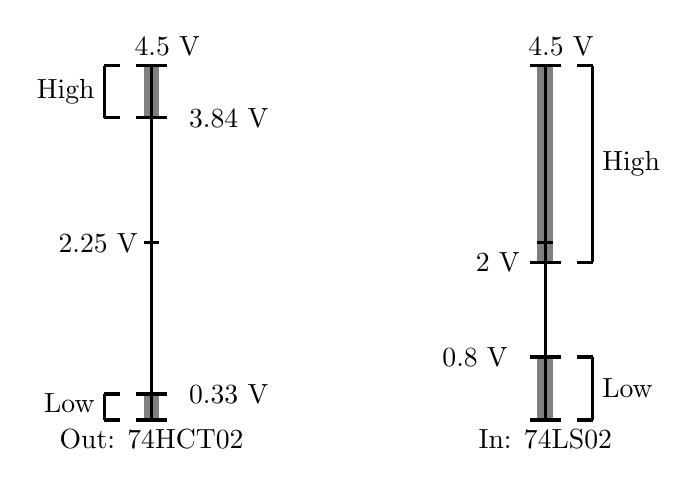
\begin{tikzpicture}[yscale=1]
	
	\node [below] at (0,0) {Out: 74HCT02};	
	
	%Límites de OUT
	\draw[-][draw=gray, line width=2mm] (0,3.84) -- (0,4.5);
	\draw[-][draw=black, very thick] (-0.2,3.84) -- (0.2,3.84)  node[label=right:3.84 V](){};
	\draw[-][draw=gray, line width=2mm] (0,0) -- (0,0.33);	
	\draw[-][draw=black, very thick] (-0.2,0.33) -- (0.2,0.33) node[label=right:0.33 V](){};

	%Eje de OUT
	\node [above] at (0.2,4.5) {4.5 V};
	\draw[-][draw=black, very thick] (0,0) -- (0,4.5);
	\draw[-][draw=black, very thick] (-0.1,2.25) -- (0.1,2.25) node[label=left:2.25 V](){};
	\draw[-][draw=black, very thick] (-0.2,0) -- (0.2,0);
	\draw[-][draw=black, very thick] (-0.2,4.5) -- (0.2,4.5);
	
	%Labels High y Low
	\draw[-][draw=black, very thick] (-0.4,4.5) -- (-0.6,4.5);
	\draw[-][draw=black, very thick] (-0.6,4.5) -- (-0.6,3.84);
	\draw[-][draw=black, very thick] (-0.4,3.84) -- (-0.6,3.84);
	\node [left] at (-0.6,4.17) {High};

	\draw[-][draw=black, very thick]	 (-0.4,0) -- (-0.6,0);
	\draw[-][draw=black, very thick]	 (-0.6,0) -- (-0.6,0.33);
	\draw[-][draw=black, very thick]	 (-0.6,0.33) -- (-0.4,0.33);
	\node [left] at (-0.6,0.215) {Low};

	%Límites de IN
	\node [below] at (5,0) {In: 74LS02};
	\draw[-][draw=gray, line width=2mm] (5,0) -- (5,0.8);
	\draw[-][draw=gray, line width=2mm] (5,2) -- (5,4.5);
	\draw[-][draw=black, very thick] (5.2,0.8) -- (4.8,0.8) node[label=left:0.8 V](){};
	\node [above] at (5.2,4.5) {4.5 V};

	%Ejes de IN y labels
	\draw[-][draw=black, very thick] (5,0) -- (5,4.5);
	\draw[-][draw=black, very thick] (4.9,2.25) -- (5.1,2.25);
	\draw[-][draw=black, very thick] (4.8,0) -- (5.2,0);
	\draw[-][draw=black, very thick] (4.8,4.5) -- (5.2,4.5);
	\draw[-][draw=black, very thick] (5.4,0) -- (5.6,0);
	\draw[-][draw=black, very thick] (4.8,2) -- (5.2,2);
	\draw[-][draw=black, very thick] (5.4,0.8) -- (5.6,0.8);
	\draw[-][draw=black, very thick] (5.6,0) -- (5.6,0.8);
	\node [right] at (5.6,0.4) {Low};

	\draw[-][draw=black, very thick] (5.4,2) -- (5.6,2);
	\node [left] at (4.8,2) {2 V};	
	\draw[-][draw=black, very thick] (5.4,4.5) -- (5.6,4.5);
	\draw[-][draw=black, very thick] (5.6,2) -- (5.6,4.5);
	\node [right] at (5.6,3.25) {High};	
\end{tikzpicture}
\end{center}
\caption{Comparación de tecnologías con HCT a la salida y LS a la entrada.}
\label{fig:hctls}
\end{figure}

\begin{figure}[H]
\begin{center}
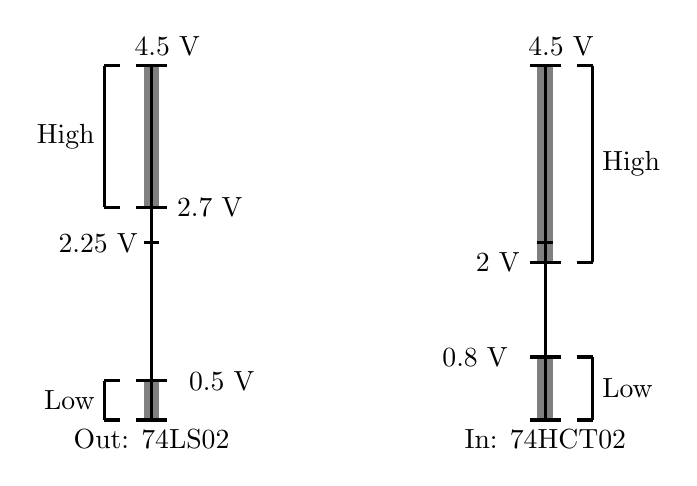
\begin{tikzpicture}[yscale=1]
	\node [below] at (0,0) {Out: 74LS02};
	
	\draw[-][draw=gray, line width=2mm] (0,2.7) -- (0,4.5);
	\draw[-][draw=gray, line width=2mm] (0,0) -- (0,0.5);	
	\draw[-][draw=black, very thick] (-0.2,2.7) -- (0.2,2.7);
	\draw[-][draw=black, very thick] (-0.2,0.5) -- (0.2,0.5) node[label=right:0.5 V](){};

	\draw[-][draw=black, very thick] (0,0) -- (0,4.5);
	\draw[-][draw=black, very thick] (-0.1,2.25) -- (0.1,2.25) node[label=left:2.25 V](){};
	\draw[-][draw=black, very thick] (-0.2,0) -- (0.2,0);
	\draw[-][draw=black, very thick] (-0.2,4.5) -- (0.2,4.5);
	
	\draw[-][draw=black, very thick] (-0.4,4.5) -- (-0.6,4.5);
	\draw[-][draw=black, very thick] (-0.6,4.5) -- (-0.6,2.7);
	\draw[-][draw=black, very thick] (-0.4,2.7) -- (-0.6,2.7);
	\node [left] at (-0.6,3.6) {High};
	\node [above] at (0.2,4.5) {4.5 V};
	
	\node [right] at (0.2,2.7) {2.7 V};
	
	\draw[-][draw=black, very thick]	 (-0.4,0) -- (-0.6,0);
	\draw[-][draw=black, very thick]	 (-0.4,0.5) -- (-0.6,0.5);
	\draw[-][draw=black, very thick]	 (-0.6,0) -- (-0.6,0.5);
	\node [left] at (-0.6,0.25) {Low};
	
	
	\node [below] at (5,0) {In: 74HCT02};
	\draw[-][draw=gray, line width=2mm] (5,0) -- (5,0.8);
	\draw[-][draw=gray, line width=2mm] (5,2) -- (5,4.5);
	\draw[-][draw=black, very thick] (5.2,0.8) -- (4.8,0.8) node[label=left:0.8 V](){};
	\node [above] at (5.2,4.5) {4.5 V};
	
	\draw[-][draw=black, very thick] (5,0) -- (5,4.5);
	\draw[-][draw=black, very thick] (4.9,2.25) -- (5.1,2.25);
	\draw[-][draw=black, very thick] (4.8,0) -- (5.2,0);
	\draw[-][draw=black, very thick] (4.8,4.5) -- (5.2,4.5);
	\draw[-][draw=black, very thick] (5.4,0) -- (5.6,0);
	\draw[-][draw=black, very thick] (5.2,2) -- (4.8,2);
	\draw[-][draw=black, very thick] (5.4,0.8) -- (5.6,0.8);
	\draw[-][draw=black, very thick] (5.6,0) -- (5.6,0.8);
	\node [right] at (5.6,0.4) {Low};

	\draw[-][draw=black, very thick] (5.4,2) -- (5.6,2);
		\draw[-][draw=black, very thick] (5.4,4.5) -- (5.6,4.5);
	\draw[-][draw=black, very thick] (5.6,2) -- (5.6,4.5);
	\node [right] at (5.6,3.25) {High};
	
	\node [left] at (4.8,2) {2 V};	
\end{tikzpicture}
\end{center}
\caption{Comparación de tecnologías con LS a la salida y HCT a la entrada.}
\label{fig:lshct}
\end{figure}

Como era de esperarse, y debido a a que la compuerta 74HCT02 es compatible con la tecnología TTL, al reemplazar la HC por la HTC se soluciona el problema presentado previamente, ya que al comparar las Figuras (\ref{fig:lshc}) y (\ref{fig:lshct}), se observa que ya no existe una zona en la cual las tensiones de salida no son consideradas como validas por la entrada siguiente.

De la misma forma que se realizó para la conexión 74HC02 - 74LS02, se mide la conexión 74HCT02 - 74LS02.
\begin{figure}[H]
\centering
	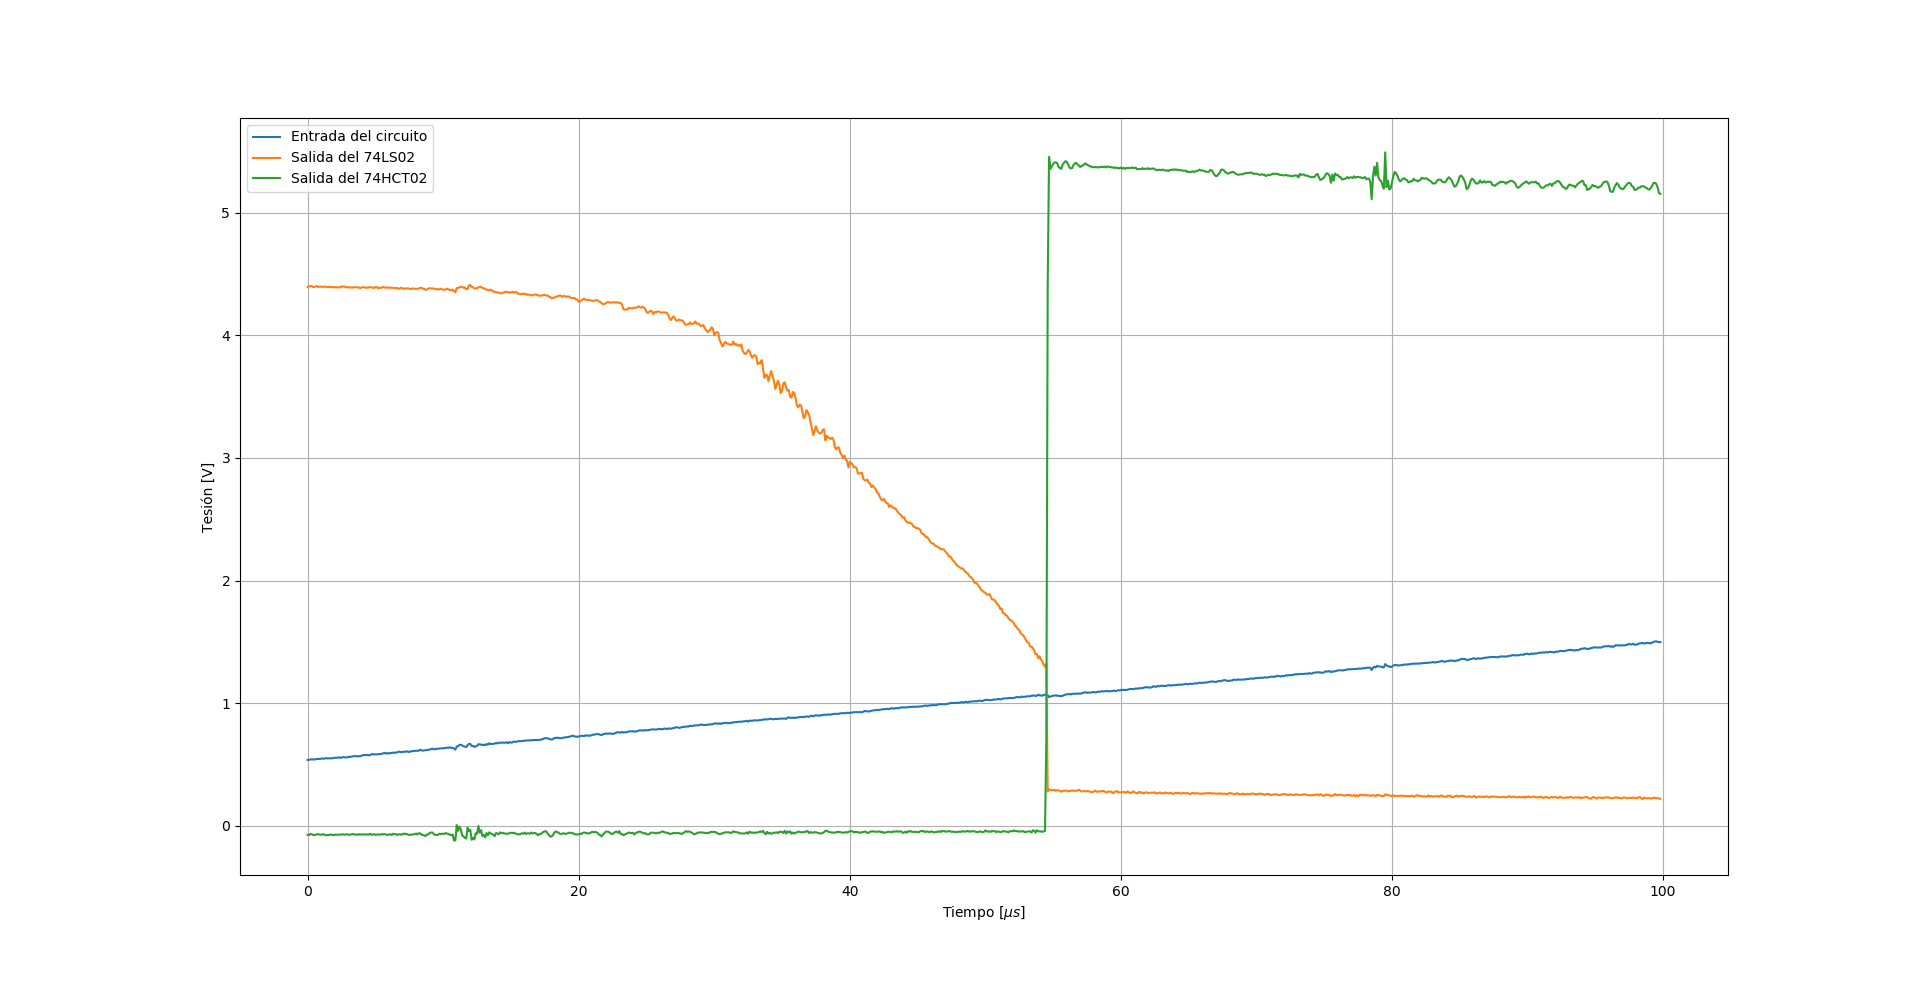
\includegraphics[width=0.8\textwidth]{ImagenesEjercicio2/scope_23_1.png}
\end{figure}
\begin{figure}[H]
\centering
	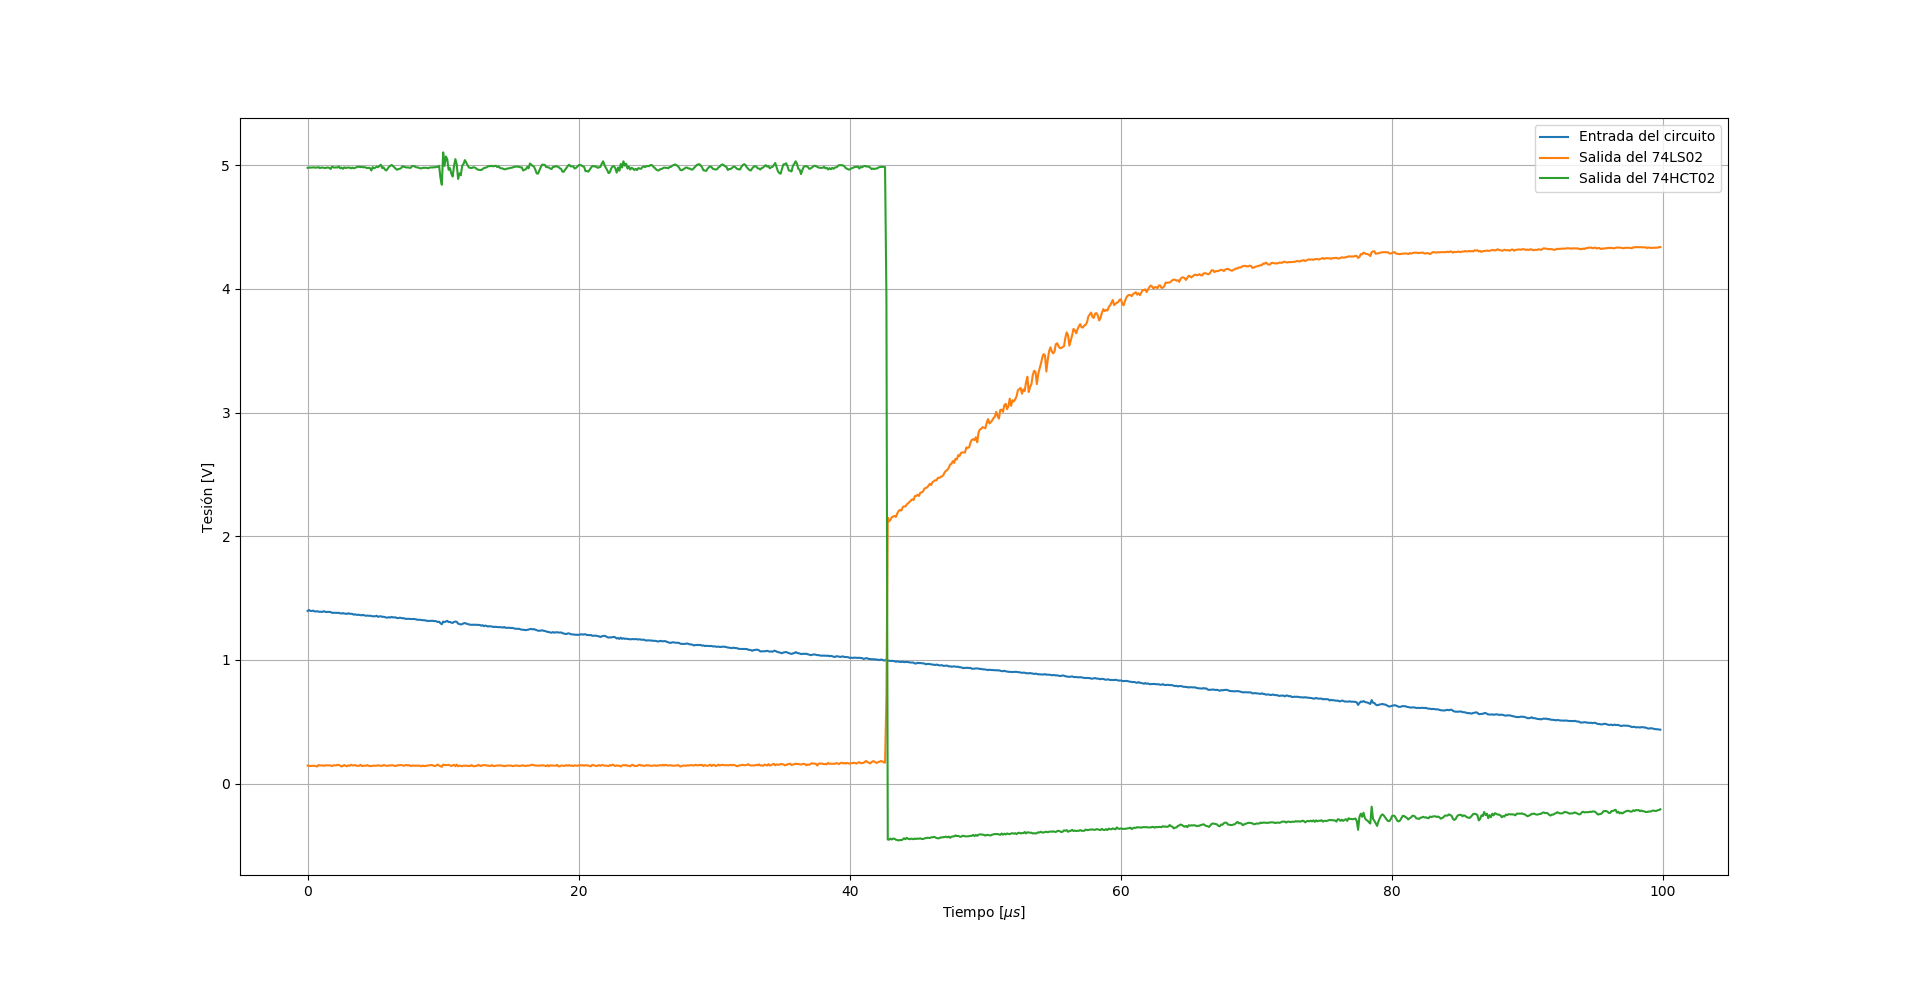
\includegraphics[width=0.8\textwidth]{ImagenesEjercicio2/scope_26_1.png}
\caption{Entrada del circuito, salida del 74LS02 y salida del 74HC02.}
\label{fig:medicion2}
\end{figure} 

Es así que comparando las Figuras (\ref{fig:medicion1}) y (\ref{fig:medicion2}), se denota como se solventa el problema existente de compatibilidad. En el segundo caso, al ser las compuertas compatibles, estas no se sobrecargan entre sí y no existen problemas de tensiones, logrando que la imagen se vea mucho mejor.

Por otro lado, se destaca que en el caso de colocar la compuerta de tecnología HCT a la salida y la LS a la entrada, no genera cambios en el fanout, ya que solo se debe corregir los valores de $I_{OH}$ y $I_{OL}$, los cuales son los mismos que para la tecnología HC.

Finalmente, se presentan las relaciones de tensiones de entrada y salida medidas, variando las combinaciones de tecnologías posibles, para las cuales se empleó el mismo suavizado exponencial para poder obtener mediciones apreciables.
\begin{figure}[H]
\centering
	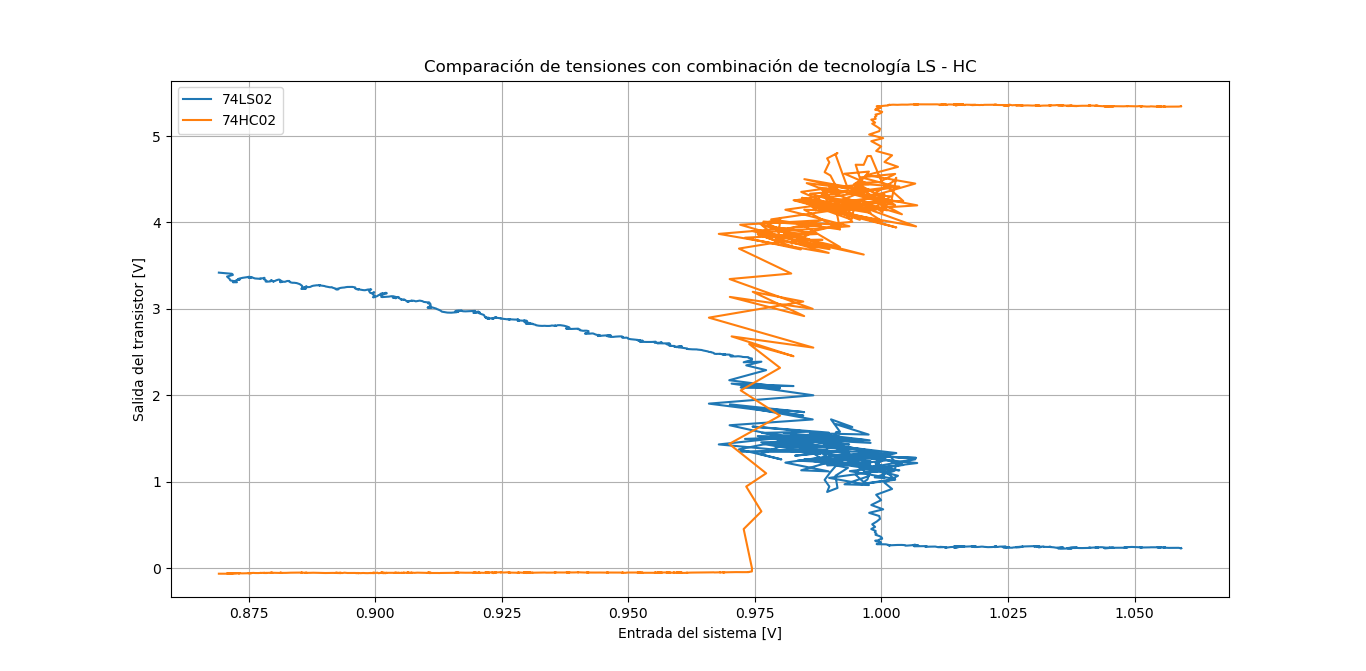
\includegraphics[width=0.8\textwidth]{ImagenesEjercicio2/Xy-feo.png}
\caption{Entradas y salidas de las compuertas con tecnologías HC y LS.}
\label{fig:xy-feo}
\end{figure}
\begin{figure}[H]
\centering
	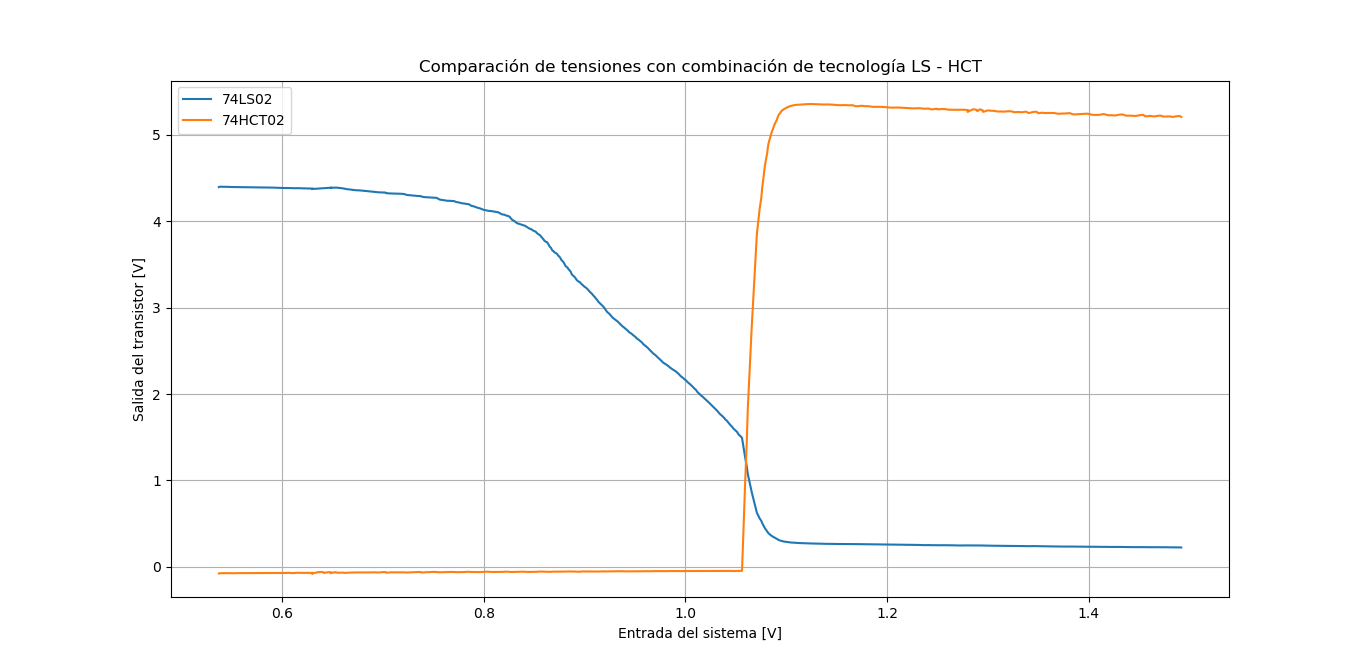
\includegraphics[width=0.8\textwidth]{ImagenesEjercicio2/Xy-bien.png}
\caption{Entradas y salidas de las compuertas con tecnologías HCT y LS.}
\label{fig:xy-bien}
\end{figure}

Se detalla de estas últimas figuras que el funcionamiento de la combinación LS - HCT, siendo el primero la salida y el segundo la entrada, es mucho más acorde y se empeña bajo un correcto funcionamiento, comparándolo con la disposición LS - HC, salida y entrada respectivamente.